\documentclass[12pt]{article}
\usepackage[paper=letterpaper,margin=2cm]{geometry}
\usepackage{amsmath}
\usepackage{amssymb}
\usepackage{amsfonts}
\usepackage{newtxtext, newtxmath}
\usepackage{enumitem}
\usepackage{titling}
\usepackage{svg}
\usepackage{xcolor}
\usepackage{listings}
\usepackage{float}
\usepackage{multicol}
\usepackage{nicefrac}
\usepackage{ragged2e}
\usepackage[autostyle]{csquotes}
\usepackage[colorlinks=true]{hyperref}

\MakeOuterQuote{"}
\setlength{\droptitle}{-6em}

\definecolor{codegreen}{rgb}{0,0.6,0}
\definecolor{codegray}{rgb}{0.5,0.5,0.5}
\definecolor{codepurple}{rgb}{0.58,0,0.82}
\definecolor{backcolour}{rgb}{0.95,0.95,0.92}

\lstdefinestyle{mystyle}{
    commentstyle=\color{codegreen},
    keywordstyle=\color{magenta},
    numberstyle=\tiny\color{codegray},
    stringstyle=\color{codepurple},
    basicstyle=\ttfamily\footnotesize,
    breakatwhitespace=false,
    breaklines=true,
    captionpos=b,
    keepspaces=true,
    numbers=left,
    numbersep=5pt,
    showspaces=false,
    showstringspaces=false,
    showtabs=false,
    tabsize=2
}

\lstset{
        style=mystyle,
        inputencoding=utf8,
        extendedchars=true,
}


\title{\large{Aprendizagem 2022}\vskip 0.2cm Homework III -- Group 019\vskip 0.2cm Diogo Gaspar 99207, Rafael Oliveira 99311}
\date{}
\begin{document}
\maketitle
\center\large{\vskip -2.5cm\textbf{Part I}: Pen and paper}
\begin{enumerate}[leftmargin=\labelsep]

  \item \textbf{Consider the basis function, $\phi_j(x) = x^j$, for performing a 3-order polynomial regression,
          $$
            \hat{z}(x, w) = \sum_{j=0}^3 w_j \phi_j(x) = w_0 + w_1 x + w_2 x^2 + w_3 x^3.
          $$
          Learn the Ridge regression ($l_2$ regularization) on the transformed data space
          using the closed-form solution with $\lambda = 2$.
        }

        We have in hands a \textbf{supervised learning} problem, with a given training
        dataset as shown below:

        \begin{table}[h]
          \centering
          \begin{tabular}{c|c|c}
                  & $y_1$ & $z$  \\ \hline
            $x_1$ & $0.8$ & $24$ \\
            $x_2$ & $1$   & $20$ \\
            $x_3$ & $1.2$ & $10$ \\
            $x_4$ & $1.4$ & $13$ \\
            $x_5$ & $1.6$ & $12$
          \end{tabular}
          \caption{Training dataset: $y_1$ as the input's (only) variable, $z$ as the target variable}
          \label{tab:training-dataset}
        \end{table}

        We can note that in the statement's estimation function, $\hat{z}(x, w)$, $x$ is a single-element vector
        (with its only entry being each sample's $y_1$ value). Therefore, it makes
        sense to "expand" the table above as follows, in order to have a broader
        representation of the values we'll end up using in the estimation function:

        \begin{table}[h]
          \centering
          \begin{tabular}{c|ccc|c}
                  & $y_1$ & $y_1^2$ & $y_1^3$ & $z$  \\ \hline
            $x_1$ & $0.8$ & $0.64$  & $0.512$ & $24$ \\
            $x_2$ & $1$   & $1$     & $1$     & $20$ \\
            $x_3$ & $1.2$ & $1.44$  & $1.728$ & $10$ \\
            $x_4$ & $1.4$ & $1.96$  & $2.744$ & $13$ \\
            $x_5$ & $1.6$ & $2.56$  & $4.096$ & $12$
          \end{tabular}
          \caption{Training dataset with additional information}
          \label{tab:expanded-training-dataset}
        \end{table}

        The equation below shows the closed-form solution for the Ridge regression
        problem, with $\lambda = 2$:

        \begin{equation*}
          % account for lambda, the bias term
          w = (\Phi^T \Phi + \lambda I)^{-1} \Phi^T z = (\Phi^T \Phi + 2 I)^{-1} \Phi^T z
        \end{equation*}

        Here, $\Phi$ is the result of applying the basis function to our training
        dataset's inputs, such that:

        \begin{equation*}
          \Phi = \begin{bmatrix}
            1      & \phi_1(x_1) & \phi_2(x_1) & \phi_3(x_1) \\
            1      & \phi_1(x_2) & \phi_2(x_2) & \phi_3(x_2) \\
            \vdots & \vdots      & \vdots      & \vdots      \\
            1      & \phi_1(x_5) & \phi_2(x_5) & \phi_3(x_5)
          \end{bmatrix} = \begin{bmatrix}
            1 & 0.8 & 0.64 & 0.512 \\
            1 & 1   & 1    & 1     \\
            1 & 1.2 & 1.44 & 1.728 \\
            1 & 1.4 & 1.96 & 2.744 \\
            1 & 1.6 & 2.56 & 4.096
          \end{bmatrix}
        \end{equation*}

        We are now able to learn the given polynomial regression model, with $\lambda = 2$:
        $$
          \begin{aligned}
            (\Phi^T \Phi + \lambda I)^{-1} & = \left(
            \begin{bmatrix}
              1 & 0.8 & 0.64 & 0.512 \\
              1 & 1   & 1    & 1     \\
              1 & 1.2 & 1.44 & 1.728 \\
              1 & 1.4 & 1.96 & 2.744 \\
              1 & 1.6 & 2.56 & 4.096
            \end{bmatrix}^T
            \begin{bmatrix}
              1 & 0.8 & 0.64 & 0.512 \\
              1 & 1   & 1    & 1     \\
              1 & 1.2 & 1.44 & 1.728 \\
              1 & 1.4 & 1.96 & 2.744 \\
              1 & 1.6 & 2.56 & 4.096
            \end{bmatrix} +
            \begin{bmatrix}
              2 & 0 & 0 & 0 \\
              0 & 2 & 0 & 0 \\
              0 & 0 & 2 & 0 \\
              0 & 0 & 0 & 2
            \end{bmatrix}
            \right)^{-1}                                                                             \\
                                           & = \begin{bmatrix}
                                                 0.34168753  & -0.1214259  & -0.07490231 & -0.00932537 \\
                                                 -0.1214259  & 0.3892078   & -0.09667718 & -0.07445624 \\
                                                 -0.07490231 & -0.09667718 & 0.37257788  & -0.17135047 \\
                                                 -0.00932537 & -0.07445624 & -0.17135047 & 0.17998796  \\
                                               \end{bmatrix}
          \end{aligned}
        $$

        \begin{equation*}
          \Phi^T z = \begin{bmatrix}
            1 & 0.8 & 0.64 & 0.512 \\
            1 & 1   & 1    & 1     \\
            1 & 1.2 & 1.44 & 1.728 \\
            1 & 1.4 & 1.96 & 2.744 \\
            1 & 1.6 & 2.56 & 4.096
          \end{bmatrix}^T
          \begin{bmatrix}
            24 \\
            20 \\
            10 \\
            13 \\
            12
          \end{bmatrix} = \begin{bmatrix}
            79      \\
            88.6    \\
            105.96  \\
            134.392 \\
          \end{bmatrix}
        \end{equation*}

        \begin{equation*}
          w = (\Phi^T \Phi + \lambda I)^{-1} \Phi^T z = \begin{bmatrix}
            7.0450759   \\
            4.64092765  \\
            1.96734046  \\
            -1.30088142 \\
          \end{bmatrix}
        \end{equation*}

        Having learned the regression model, we can now use it to predict labels $z$
        for new samples!

        \pagebreak

  \item \textbf{Compute the training RMSE for the learnt regression model.}

        \pagebreak

  \item \textbf{Consider a multi-layer perceptron characterized by one hidden layer with 2 nodes.
          Using the activation function $f(x) = e^{0.1x}$ on all units, all weights
          initialized as 1 (including biases), and the half squared error loss, perform
          one batch gradient descent update (with learning rate $\eta = 0.1$)
          for the first three observations (0.8), (1) and (1.2).
        }

\end{enumerate}

\pagebreak

\center\large{\textbf{Part II}: Programming and critical analysis}

\begin{justify}
  The code utilized to answer the following questions is available in this
  report's appendix.
\end{justify}

\begin{enumerate}[leftmargin=\labelsep,resume]
  \item \textbf{Compute the MAE of the three regressors: linear regression, $MLP_1$ and $MLP_2$.}

        We opted to utilize \texttt{sklearn}'s \texttt{mean\_absolute\_error} function to compute the MAE of the three regressors.
        The regressors were created as shown in the appendix (using \texttt{Ridge} and
        \texttt{MLPRegressor} with the respective parameters).

        We gathered the following results:

        \begin{table}[h]
          \centering
          \begin{tabular}{l|l}
            Regressor                 & MAE       \\ \hline
            Linear Regression (Ridge) & $0.16283$ \\
            $MLP_1$                   & $0.06804$ \\
            $MLP_2$                   & $0.09781$
          \end{tabular}
          \caption{Gathered Mean Absolute Errors for each specified regressor}
          \label{tab:mean-absolute-errors}
        \end{table}

  \item \textbf{Plot the residues (in absolute value) using two visualizations: boxplots and histograms.}

        Each regressor's residues, calculated as the absolute difference between
        the predicted and actual values, were plotted using both boxplots and histograms
        (using, respectively, \texttt{seaborn}'s \texttt{boxplot} and \texttt{histplot} functions),
        as shown in this report's appendix (figures after the code).

  \item \textbf{How many iterations were required for $MLP_1$ and $MLP_2$ to converge?}

        Calling the \texttt{print\_regressor} method for each regressor shows us
        not only the MAE, but also the number of iterations required for each of
        the MLP regressors to converge. In this case, the number of iterations
        required for $MLP_1$ ($MLP$ with early stopping) to converge was 452,
        while $MLP_2$ ($MLP$ \textit{without} early stopping) required only 77.

  \item \textbf{What can be motivating the unexpected differences on the number of iterations?
          Hypothetize one reason underlying the observed performance differences between the MLPs.}
\end{enumerate}

\pagebreak

\large{\textbf{Appendix}\vskip 0.3cm}

\lstinputlisting[language=Python]{code.py}

% TODO: figures should be presented neatly, currently aren't

\begin{figure}[h]
  \centering
  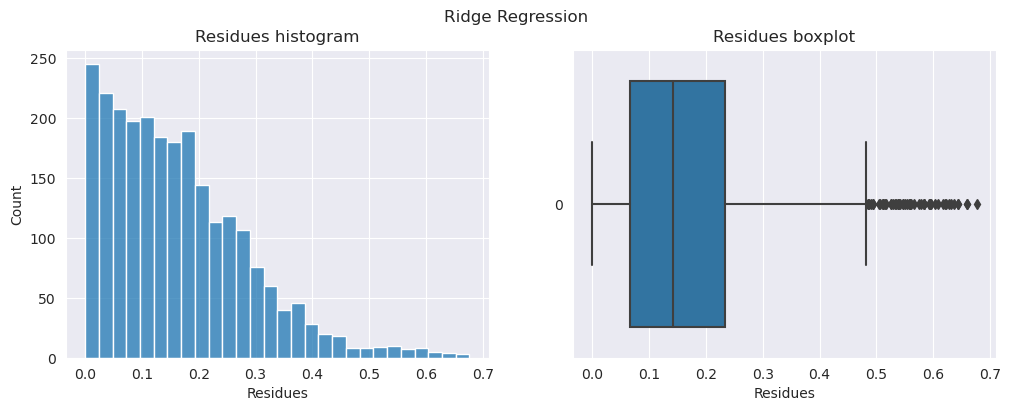
\includegraphics[width=\textwidth]{../assets/ridge-plots.png}
  \caption{Ridge regression's residue plotting}
  \label{fig:ridge-plotting}
\end{figure}

\begin{figure}[h]
  \centering
  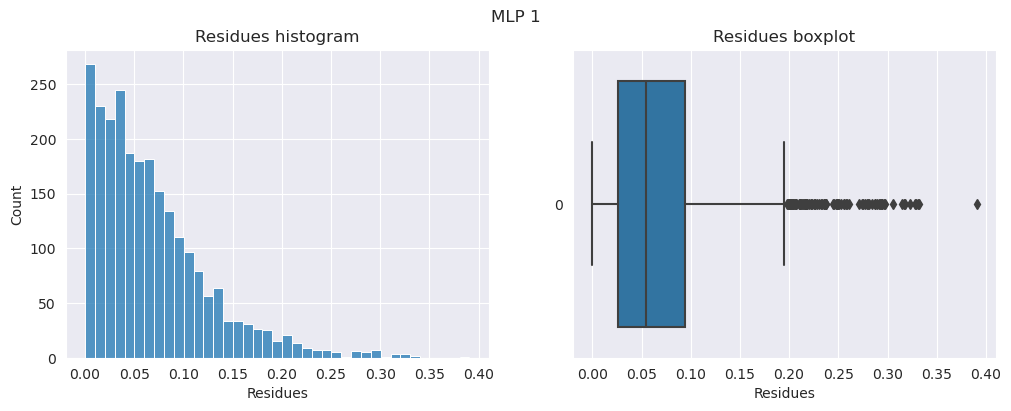
\includegraphics[width=\textwidth]{../assets/mlp1-plots.png}
  \caption{$MLP_1$ regression's residue plotting}
  \label{fig:mlp1-plotting}
\end{figure}

\begin{figure}[h]
  \centering
  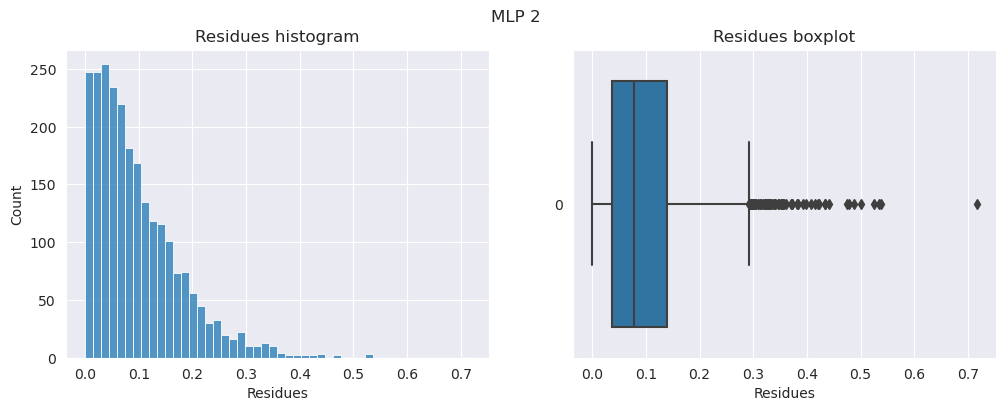
\includegraphics[width=\textwidth]{../assets/mlp2-plots.png}
  \caption{$MLP_2$ regression's residue plotting}
  \label{fig:mlp2-plotting}
\end{figure}

\end{document}
